\documentclass[a4paper]{article}
\usepackage[a4paper,  margin=1.0in]{geometry}

\usepackage{graphicx}
\usepackage{float}
\usepackage{hyperref}
\usepackage{listings}
\lstset{
basicstyle=\small\ttfamily,
columns=flexible,
breaklines=true
}

\usepackage{polski}
\usepackage[utf8]{inputenc}
\begin{document}


\title{Ćwiczenie nr 3 z MBI, Resekwencjonowanie genomu człowieka}
\author{Kinga Kimnes, Jakub Skałecki}
\maketitle

W ramach przeprowadzanego ćwiczenia wykorzystano plik FASTA zawierający fragment ludzkiego genomu referencyjnego (GRCh37) uzyskanego przez Human Genome Consortium w 2009 roku. Plik ten zawiera sekwencję chromosomu 1.

\section{Mapowanie}


Początkowo dokonano indeksowania pliku FASTA poprzez zastosowanie programu BWA (Burrows-Wheeler Alignment Tool).
Jest on stosowany do mapowania sekwencji o małej rozbieżności względem duzego genomu referencyjnego, takiego jak genom ludzki.
Pakiet BWA składa się z trzech algorytmów: BWA-backtrack, BWA-SW oraz BW-MEM, przy czym dla zapytań o wysokiej jakości zalecany jest ostatni z nich z uwagi na wydajność i dokładność.
Następnie, za pomocą ostatniego ze wskazanych algorytmów - BWA-MEM, wygenerowano plik SAM (Sequence Alignment/Map) zawierający mapowania kolejnych sekwencji z pliku coriell\_chr1.fq na sekwencję referencyjną, którą stanowił plik chr1.fa (sekwencja chromosomu 1).

Typowa (średnia) długość odczytu to 75.5bp, o odchyleniu standardowym równym około 1.17.
W dalszej kolejności dokonano sortowania mapowań oraz wygenerowano plik BAM (Binary Alignment/Map - stanowiący binarny odpowiednik pliku SAM). Rozmiary plików wynosiły kolejno: FASTQ-57MB, SAM - 77MB, BAM - 14MB.

Plik FASTQ zawiera sekwencje (odczyty) oraz zapisaną symbolicznie ocenę jakości dla każdego nukleotydu (ilość równa długości sekwencji). Plik SAM zawiera ponadto informacje o mapowaniu sekwencji na genom referencyjny, co czyni go większym.

\section{Wizualizacja przykładowego wariantu w genie IQGAP3}

Przykładowy wariant ma pozycję 156,498,673 i jest wariantem homozygotycznym. Genom referencyjny zawiera nukleotyd T, a odczyty wskazują A. Zrzut ekranu znajduje się na rysunku \ref{fig:igv}.

\begin{figure}[h]
    \centering
    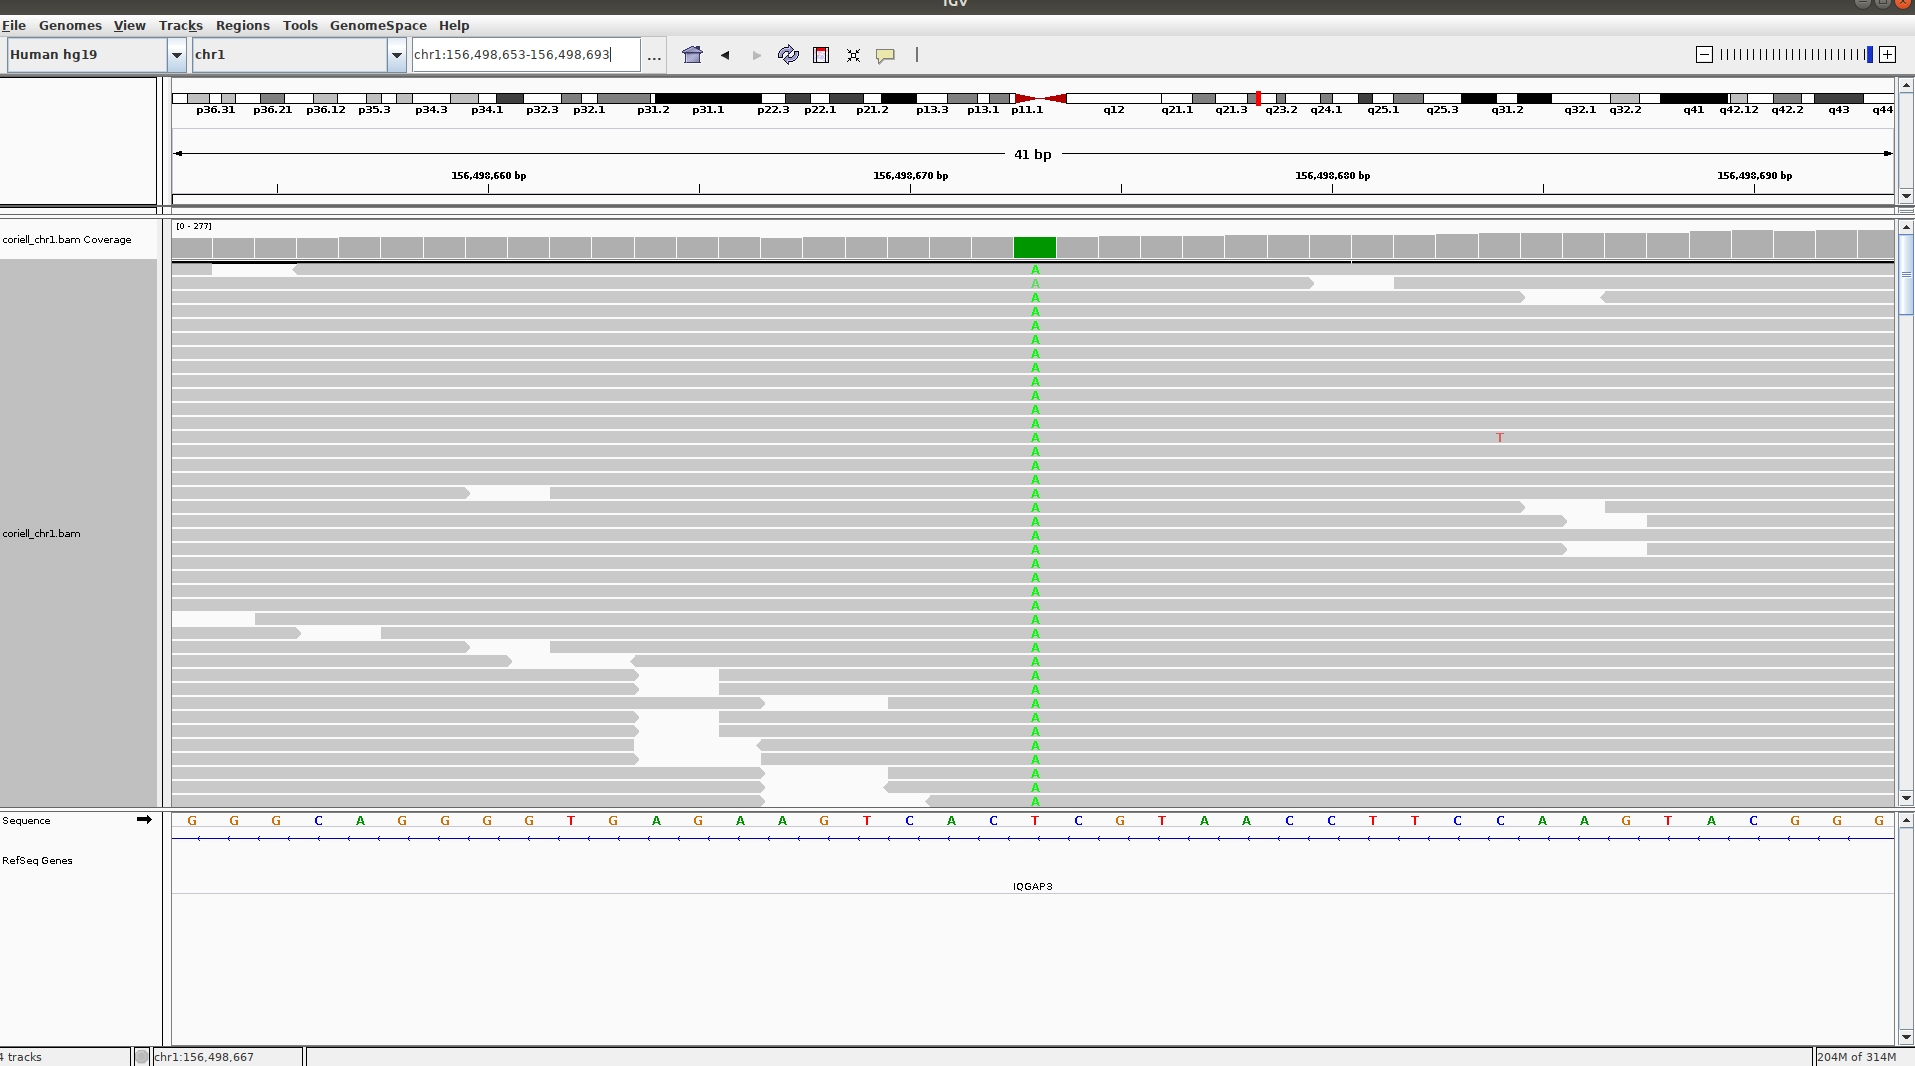
\includegraphics[width=1.0\textwidth]{vcf.png}
    \label{fig:igv}
    \caption[]{Przykładowy wariant w oknie IGV}
\end{figure}


\section{Wykrywanie wariantów}

Ilość wariantów bez filtracji to 6050, po odfiltrowaniu wariantów z pokryciem mniejszym niż 11 zostało ich 241. Dalsza filtracja może odbyć się po np INFO/MQ - średnia jakość mapowania.

\section{Adnotacje wariantów}
W wyniku przeprowadzonej za pomocą narzędzia Variant Effect Predictor adnotacji przefiltorwanego pliku VCF uzyskano wykres typu "pie chart" przedstawiający statystyki wariantów. Największy udział procentowy posiada intron\_variant (36\%). Odpowiadające mu wiersze zamieszczono w tabeli \ref{table:3lines}.

\begin{table}[H]
    \caption{
    \label{table:3lines}
    }
\begin{center}
\begin{tabular}{| p{150mm} |}

    \hline
    \verb|.	.	1:156498673-156498673	A	intron_variant	MODIFIER	IQGAP3	ENSG00000183856	Transcript	ENST00000361170.2	protein_coding	- 35/37	-	-	-	-	-	-	-	rs1171564	-	-1	-	HGNC	20669	-	-	-	-	-	0.5998	-	-	-	-	-	-	-	-|
    \\
    \hline
\verb|.	1:156498673-156498673	A	upstream_gene_variant	MODIFIER	snoU13	ENSG00000238843	Transcript	ENST00000458777.1	snoRNA	-	-	-	-	-	-	-	-	-	rs1171564	449	1	-	RFAM	-	-	-	-	-	-	0.5998	-	-	-	-	-	-	-	-|
    \\
    \hline
\verb|.	1:156498673-156498673	A	intron_variant,NMD_transcript_variant	MODIFIER	IQGAP3	ENSG00000183856	Transcript	ENST00000491900.1	nonsense_mediated_decay	-	34/37	-	-	-	-	-	-	-	rs1171564	-	-1	-	HGNC	20669	-	-	-	-	-	0.5998	-	-	-	-	-	-	-	-|
    \\
    \hline
\end{tabular}
\end{center}
\end{table}

Jest to wariant w sekwencji niekodującej (o czym świadczy wartość w kolumnie Intron (35/37) oraz Consequence (intron\_variant)) w pierwszym wierszu powyższego listingu.

\section{Wnioski}
Celem ćwiczenia była analiza danych z resekwencjonowania fragmentu genomu ludzkiego, a  materiał badawczy stanowiła sekwencja chromosomu 1. W wyniku mapowania tejże sekwencji do genomu referencyjnego uzsykano dodatkowe informacje w postaci dopasowanych (wykrytych) wariantów - plik SAM.W celu zwizualizowania uzyskanych danych, wykorzystano program IGV, do którego załadowano binarny odpowiednik tego pliku. Otrzymane dane umożliwiają zarówno weryfikację różnic w stosunku do genomu referencyjnego, jak i pomiar tej różnicy (liczba nukleotydów oznaczonych jako inne niż referencyjne, zsumowana dla wszystkich pokryć). Raport wygenerowany w oparciu o przefiltrowany plik VCF za pomocą narzędzia VEP pozwolił na określenie typu adnotowanych wariantów. Duża część z nich występuje w intronach (sekwencjach niekodujących - 36\%) i transkryptach niekodujących (10\%). Pośród sekwencji kodujących, największą część stanowią warianty równoznaczne (57\%) - w których nie następuje żadna zmiana kodowanego aminokwasu.
\end{document}
